\section{Experimental Evaluation}\label{sec:experiment}

In this section, we implement \chatiot\ and conduct extensive evaluation. 
We study the effectiveness of \chatiot\ and answer the following questions:

\noindent \textbf{Q1:} How does \datakit\ extract appropriate field selection from IoT threat datasets and convert them into well-structured documents for retrieval and LLM analysis?
What are the optimal chunking strategies for each kind of document? (\S~\ref{sec:exp-dataprocess})

\noindent \textbf{Q2:} What are the advantages of our system? Can \chatiot\ effectively generalize and improve the capabilities of the most advanced LLMs available in processing IoT security issues? (\S~\ref{sec:exp-llmeval})

\noindent \textbf{Q3:} Can \chatiot\ be a practical useful IoT assistant over using LLM alone? How about the feedback from real-world human evaluation? (\S~\ref{sec:exp-human})


\subsection{Setup}
\noindent \textbf{Testbed.}
We implement \chatiot\ in Python 3.10.13, utilizing large language models LLaMA3:8B \& 70B and LLaMA3.1:8B \& 70B provided by Groq\footnote{\scriptsize \url{https://chat.groq.com/}}, GPT-4o-mini and 4o provided by OpenAI\footnote{\scriptsize \url{https://platform.openai.com/docs/models/gpt-4o}}. All these LLMs are utilized by calling their APIs.
For building the vector store, we employed Elasticsearch 8.13.2~\cite{elasticsearch2018elasticsearch}, running on Docker Desktop 4.29.0~\cite{docker-desktop}. 
All components were integrated using the LangChain library (version 0.2.5)~\cite{langchain2024}. 
The WebApp was developed using Streamlit (version 1.33.0)~\cite{streamlit}. 
Experiments were conducted on a MacBook Pro equipped with an Apple M3 Pro CPU (11 cores) and 18 GB of RAM, running macOS 14.6.1 with the Darwin 23.6.0 kernel.

\smallskip
\noindent \textbf{Data Sources.}
We collect five kinds of IoT security and threat datasets from the public Internet:
\begin{itemize}
\item[\romannumeral1)] VARIoT vulnerabilities~\cite{VARIoT_db}: This dataset catalogs known vulnerabilities in various IoT devices, offering detailed information about the potential risks associated with each vulnerability.
\item[\romannumeral2)] VARIoT exploits~\cite{VARIoT_db}: This dataset contains exploits targeting IoT devices, providing insights into the techniques and methods attackers use to compromise these systems.
\item[\romannumeral3)] MITRE ATT\&CK ICS TTPs~\cite{strom2018mitre}: This dataset outlines the tactics, techniques, and procedures (TTPs) employed by adversaries specifically in industrial control systems (ICS), which often include IoT-related TTPs as well.
\item[\romannumeral4)] Threat reports: We collect $17$ public threat reports from VXUG\footnote{\scriptsize \url{https://vx-underground.org/}} about emerging threats and vulnerabilities, offering analysis and recommendations for mitigating potential risks.
\item[\romannumeral5)] Cybersecurity labelling schemes\footnote{\scriptsize \url{https://www.csa.gov.sg/our-programmes/certification-and-labelling-schemes}}\footnote{\scriptsize \url{https://tietoturvamerkki.fi/en/products}}
\footnote{\scriptsize \url{https://www.nemko.com}}
\footnote{\scriptsize \url{https://nvlpubs.nist.gov/nistpubs/CSWP/NIST.CSWP.02042022-2.pdf}}: These schemes provide information on the security posture of various IoT products, helping consumers and organizations assess the security standards and certifications achieved by specific devices.
\end{itemize}
These datasets provide comprehensive insights into the current landscape of IoT threats, enabling us to enhance our system's capabilities.


%For each user case defined in \S~\ref{sec:usecase}, we propose 10 queries. 
%Then, we compare the generated answers of \chatiot\ with those generated by only using the corresponding LLM without augmented retrieval.
%and the commercial LLMs such as OpenAI ChatGPT3.5 and Google Gemini, to illustrate our improvements in IoT security.


\subsection{Fields Selection \& Chunking Strategy}\label{sec:exp-dataprocess}

This section shows the experimental evaluation for field selection and chunking strategy optimization.

\begin{table}[h]
    \centering
    \caption{Large Language Models-based field selection for page\_content and metadata. \ding{52} is for page\_content, $\bigcirc$ denotes metadata, and \ding{56} indicates unused fields.}
    \label{tab:fieldsel-eva}
    \resizebox{0.48\textwidth}{!}{
    \begin{tabular}{c|c|ccc}
    \toprule
    \toprule
    {Dataset} & {Fields} & {\footnotesize LLaMA3:8B} & {\footnotesize LLaMA3.1:70B} & {\footnotesize GPT-4o} \\ \midrule
    \multirow{12}{*}{\rotatebox{90}{VARIoT Vulnerabilities}} 
    & \texttt{cve} & \ding{56}  &$\bigcirc$ &  $\bigcirc$\\ 
    &\texttt{id} & $\bigcirc$ &$\bigcirc$ & $\bigcirc$\\ 
    &\texttt{credit} & \ding{52} & \ding{56} & $\bigcirc$\\ 
    &\texttt{description} & \ding{52} & \ding{52} & \ding{52} \\ 
    &\texttt{title} & \ding{52} & \ding{52} & \ding{52} \\ 
    &\texttt{products} & $\bigcirc$ &$\bigcirc$ & $\bigcirc$ \\ 
    &\texttt{vulns.-config.} & $\bigcirc$ & \ding{52} & $\bigcirc$ \\ 
    &\texttt{cvss-score} & \ding{56} & \ding{56} & $\bigcirc$ \\ 
    &\texttt{cvss-string} & \ding{56} & $\bigcirc$ & \ding{52} \\ 
    &\texttt{reference} & \ding{56} & \ding{52} & \ding{52} \\ 
    &\texttt{published} & \ding{56} & $\bigcirc$ & \ding{56} \\ 
    &\texttt{modified} & \ding{56} & $\bigcirc$ & \ding{56}\\ 
    \midrule
    \multirow{8}{*}{\rotatebox{90}{VARIoT Exploit}} 
    & \texttt{id} & $\bigcirc$ & $\bigcirc$ & $\bigcirc$ \\ 
    &\texttt{credit} & \ding{56} & $\bigcirc$ & $\bigcirc$ \\
    &\texttt{description} & \ding{52} & \ding{52} & \ding{52}\\
    &\texttt{exploit} & \ding{52} & \ding{52} & \ding{52}\\
    &\texttt{title} & \ding{52} & \ding{52} & \ding{52} \\
    &\texttt{cve-id} & $\bigcirc$ & $\bigcirc$ & $\bigcirc$ \\
    &\texttt{reference} & \ding{56} & $\bigcirc$ & \ding{52} \\
    &\texttt{products} & $\bigcirc$ & $\bigcirc$ & $\bigcirc$ \\
    \midrule
    \multirow{12}{*}{\rotatebox{90}{MITRE ATT\&CK ICS}} 
    &\texttt{stixId} & $\bigcirc$ & $\bigcirc$ & $\bigcirc$ \\
    &\texttt{name} & \ding{52} & \ding{52} & \ding{52} \\
    &\texttt{parentName} & \ding{52} & \ding{56} & \ding{52} \\
    &\texttt{description} & \ding{52} & \ding{52} & \ding{52} \\
    &\texttt{lunrRef} & \ding{56} & \ding{56} & $\bigcirc$ \\
    &\texttt{id} & $\bigcirc$ & \ding{56} & $\bigcirc$ \\
    &\texttt{url} & \ding{56} & \ding{56} & \ding{56} \\
    &\texttt{is\_enterprise} & \ding{56} & $\bigcirc$ & $\bigcirc$ \\
    &\texttt{type} & \ding{56} & $\bigcirc$ & $\bigcirc$ \\
    &\texttt{relatedTech.} & \ding{56} & $\bigcirc$ & \ding{56} \\
    &\texttt{is\_ics} & \ding{56} & \ding{56} & \ding{56} \\
    &\texttt{deprecated} & \ding{56} & \ding{56} & $\bigcirc$ \\
    \bottomrule
    \bottomrule
\end{tabular}}
\end{table}

\subsubsection{Fields for Page\_Content \& Metadata}\label{sec:exp-field}
Recall that for each dataset, we should first determine the fields for page\_content and metadata for documents before building self-querying retrievers (see \S~\ref{sec:toolkit}).
For each dataset, we sample 3 items, list the fields' names, and instruct the LLM to select the suitable fields. The results are as follows:
\begin{itemize}
    \item We use three LLMs: LLaMA3:8B, LLaMA3.1:70B, and GPT4-o, to select fields for VARIoT vulnerabilities, exploits, and MITRE ATT\&CK ICS.
    The experimental results are summarized in Table~\ref{tab:fieldsel-eva}.
    While there are slight variations in their selections, there is consensus on the crucial decisions:
    For instance, in the case of the VARIoT vulnerabilities, all LLMs select \texttt{title} and \texttt{description} for page\_content, and \texttt{id} and \texttt{products} for metadata.
    Similar selections are observed for the VARIoT exploits and MITRE ATT\&CK ICS datasets.

    \item For threat reports, which are typically unstructured, we use the report's content as page\_content and the title as metadata (Note we do not use self-querying retrieval for threat reports). 
    The CLS schemes consist solely of metadata with no descriptive content, so we leave page\_content blank and utilize the metadata for self-querying retrievers.
\end{itemize}
The specific fields selected for page\_content and metadata are detailed in Table~\ref{tab:fieldselect}.


\begin{table}[]
    \centering
    \caption{Selected fields for page\_content and metadata of each dataset used in \chatiot.}
    \label{tab:fieldselect}
    \resizebox{0.48\textwidth}{!}{
    \begin{tabular}{@{}c@{\hskip 0.1cm}|@{\hskip 0.1cm}>{\centering\arraybackslash}p{4cm}@{\hskip 0.1cm}|@{\hskip 0.1cm}>{\centering\arraybackslash}p{2cm}@{\hskip 0.1cm}}
    \toprule \toprule
         {Dataset} & {Page\_content} & {Metadata}  \\ \midrule
         {\scriptsize {VARIoT Vulns.}} & {\scriptsize {\texttt{title}, \texttt{description}}} & {\scriptsize {\texttt{id}, \texttt{products}}}\\ \hline 
         {\scriptsize{VARIoT Exps.}} & {\scriptsize {\texttt{title}, \texttt{description}, \texttt{exploit}}} & {\scriptsize {\texttt{id}, \texttt{products}}} \\ \hline
         {\scriptsize{ICS}} & {\scriptsize {\texttt{name}, \texttt{description}}} & {\scriptsize {\texttt{stixId}}} \\ \hline
         {\scriptsize{Threat Report}} & {\scriptsize {\texttt{Report's content}}} & {\scriptsize \texttt{title}} \\ \hline
         {\scriptsize{CLS}} & {\scriptsize \texttt{NULL}} & {\scriptsize {\texttt{All Fields}}} \\
         \bottomrule \bottomrule
    \end{tabular}}
\end{table}


\subsubsection{Chunking Evaluation}\label{sec:exp-chunk}

%\begin{table}[htbp]
\centering
\caption{VARIoT Vulnerabilities: Precision (p) and Recall (r) for Different Chunking Strategies.}
\resizebox{0.5\textwidth}{!}{
\begin{tabular}{c|c|c|c}
\toprule
\textbf{(Size, Overlap)} & \textbf{Character} & \textbf{RecursiveCharacter} & \textbf{TokenText} \\
\midrule
(500, 50)  & (0.8747, 0.9059) & (0.9813, 0.8976) & (0.9358, 0.8957) \\
(500, 100) & (0.8764, 0.9214) & (0.9864, 0.9733) & (0.9019, 0.9428) \\
(500, 150) & (0.9167, 0.9092) & (0.9830, 0.9547) & (0.9291, 0.9298) \\
(500, 200) & (0.9288, 0.9194) & (0.9133, 0.9347) & (0.9371, 0.8971) \\
\midrule
(1000, 50)  & (0.9045, 0.8674) & (0.9549, 0.8916) & (0.9149, 0.9024) \\
(1000, 100) & (0.8826, 0.8834) & (0.9259, 0.9187) & (0.8808, 0.8434) \\
(1000, 150) & (0.8907, 0.8973) & (0.9164, 0.9585) & (0.8916, 0.8735) \\
(1000, 200) & (0.8914, 0.9178) & (0.9125, 0.9299) & (0.8993, 0.8936) \\
\midrule
(1500, 50)  & (0.8947, 0.8821) & (0.8929, 0.9222) & (0.9182, 0.8294) \\
(1500, 100) & (0.8832, 0.8814) & (0.8894, 0.8817) & (0.8875, 0.8655) \\
(1500, 150) & (0.8944, 0.8546) & (0.9132, 0.8522) & (0.8912, 0.8475) \\
(1500, 200) & (0.8417, 0.8464) & (0.9220, 0.8959) & (0.8929, 0.8033) \\
\midrule
(2000, 50)  & (0.9291, 0.8941) & (0.9131, 0.8862) & (0.8987, 0.8414) \\
(2000, 100) & (0.9028, 0.8352) & (0.8864, 0.8817) & (0.8785, 0.8655) \\
(2000, 150) & (0.9132, 0.8531) & (0.8611, 0.8839) & (0.9164, 0.8543) \\
(2000, 200) & (0.8593, 0.8812) & (0.9065, 0.9058) & (0.9226, 0.8306) \\
\bottomrule
\end{tabular}
}
\end{table}

\begin{table}[htbp]
\centering
\caption{VARIoT Vulnerabilities: Precision (p) and Recall (r) for Different Chunking Strategies.}
\resizebox{0.5\textwidth}{!}{
\begin{tabular}{c|c|c|c}
\toprule
\textbf{(Size, Overlap)} & \textbf{Character} & \textbf{RecursiveCharacter} & \textbf{TokenText} \\
\midrule
(500, 50)  & (0.8747, 0.9059) & (0.9813, 0.8976) & (0.9358, 0.8957) \\
(500, 100) & (0.8764, 0.9214) & (0.9864, 0.9733) & (0.9019, 0.9428) \\
(500, 150) & (0.9167, 0.9092) & (0.9830, 0.9547) & (0.9291, 0.9298) \\
(500, 200) & (0.9288, 0.9194) & (0.9133, 0.9347) & (0.9371, 0.8971) \\
\midrule
(1000, 50)  & (0.9045, 0.8674) & (0.9549, 0.8916) & (0.9149, 0.9024) \\
(1000, 100) & (0.8826, 0.8834) & (0.9259, 0.9187) & (0.8808, 0.8434) \\
(1000, 150) & (0.8907, 0.8973) & (0.9164, 0.9585) & (0.8916, 0.8735) \\
(1000, 200) & (0.8914, 0.9178) & (0.9125, 0.9299) & (0.8993, 0.8936) \\
\midrule
(1500, 50)  & (0.8947, 0.8821) & (0.8929, 0.9222) & (0.9182, 0.8294) \\
(1500, 100) & (0.8832, 0.8814) & (0.8894, 0.8817) & (0.8875, 0.8655) \\
(1500, 150) & (0.8944, 0.8546) & (0.9132, 0.8522) & (0.8912, 0.8475) \\
(1500, 200) & (0.8417, 0.8464) & (0.9220, 0.8959) & (0.8929, 0.8033) \\
\midrule
(2000, 50)  & (0.9291, 0.8941) & (0.9131, 0.8862) & (0.8987, 0.8414) \\
(2000, 100) & (0.9028, 0.8352) & (0.8864, 0.8817) & (0.8785, 0.8655) \\
(2000, 150) & (0.9132, 0.8531) & (0.8611, 0.8839) & (0.9164, 0.8543) \\
(2000, 200) & (0.8593, 0.8812) & (0.9065, 0.9058) & (0.9226, 0.8306) \\
\bottomrule
\end{tabular}
}
\end{table}

\begin{table}[htbp]
\centering
\caption{VARIoT Vulnerabilities: Precision (p) and Recall (r) for Different Chunking Strategies.}
\resizebox{0.5\textwidth}{!}{
\begin{tabular}{c|c|c|c}
\toprule
\textbf{(Size, Overlap)} & \textbf{Character} & \textbf{RecursiveCharacter} & \textbf{TokenText} \\
\midrule
(500, 50)  & (0.8747, 0.9059) & (0.9813, 0.8976) & (0.9358, 0.8957) \\
(500, 100) & (0.8764, 0.9214) & (0.9864, 0.9733) & (0.9019, 0.9428) \\
(500, 150) & (0.9167, 0.9092) & (0.9830, 0.9547) & (0.9291, 0.9298) \\
(500, 200) & (0.9288, 0.9194) & (0.9133, 0.9347) & (0.9371, 0.8971) \\
\midrule
(1000, 50)  & (0.9045, 0.8674) & (0.9549, 0.8916) & (0.9149, 0.9024) \\
(1000, 100) & (0.8826, 0.8834) & (0.9259, 0.9187) & (0.8808, 0.8434) \\
(1000, 150) & (0.8907, 0.8973) & (0.9164, 0.9585) & (0.8916, 0.8735) \\
(1000, 200) & (0.8914, 0.9178) & (0.9125, 0.9299) & (0.8993, 0.8936) \\
\midrule
(1500, 50)  & (0.8947, 0.8821) & (0.8929, 0.9222) & (0.9182, 0.8294) \\
(1500, 100) & (0.8832, 0.8814) & (0.8894, 0.8817) & (0.8875, 0.8655) \\
(1500, 150) & (0.8944, 0.8546) & (0.9132, 0.8522) & (0.8912, 0.8475) \\
(1500, 200) & (0.8417, 0.8464) & (0.9220, 0.8959) & (0.8929, 0.8033) \\
\midrule
(2000, 50)  & (0.9291, 0.8941) & (0.9131, 0.8862) & (0.8987, 0.8414) \\
(2000, 100) & (0.9028, 0.8352) & (0.8864, 0.8817) & (0.8785, 0.8655) \\
(2000, 150) & (0.9132, 0.8531) & (0.8611, 0.8839) & (0.9164, 0.8543) \\
(2000, 200) & (0.8593, 0.8812) & (0.9065, 0.9058) & (0.9226, 0.8306) \\
\bottomrule
\end{tabular}
}
\end{table}

\begin{table}[htbp]
\centering
\caption{VARIoT Vulnerabilities: Precision (p) and Recall (r) for Different Chunking Strategies.}
\resizebox{0.5\textwidth}{!}{
\begin{tabular}{c|c|c|c}
\toprule
\textbf{(Size, Overlap)} & \textbf{Character} & \textbf{RecursiveCharacter} & \textbf{TokenText} \\
\midrule
(500, 50)  & (0.8747, 0.9059) & (0.9813, 0.8976) & (0.9358, 0.8957) \\
(500, 100) & (0.8764, 0.9214) & (0.9864, 0.9733) & (0.9019, 0.9428) \\
(500, 150) & (0.9167, 0.9092) & (0.9830, 0.9547) & (0.9291, 0.9298) \\
(500, 200) & (0.9288, 0.9194) & (0.9133, 0.9347) & (0.9371, 0.8971) \\
\midrule
(1000, 50)  & (0.9045, 0.8674) & (0.9549, 0.8916) & (0.9149, 0.9024) \\
(1000, 100) & (0.8826, 0.8834) & (0.9259, 0.9187) & (0.8808, 0.8434) \\
(1000, 150) & (0.8907, 0.8973) & (0.9164, 0.9585) & (0.8916, 0.8735) \\
(1000, 200) & (0.8914, 0.9178) & (0.9125, 0.9299) & (0.8993, 0.8936) \\
\midrule
(1500, 50)  & (0.8947, 0.8821) & (0.8929, 0.9222) & (0.9182, 0.8294) \\
(1500, 100) & (0.8832, 0.8814) & (0.8894, 0.8817) & (0.8875, 0.8655) \\
(1500, 150) & (0.8944, 0.8546) & (0.9132, 0.8522) & (0.8912, 0.8475) \\
(1500, 200) & (0.8417, 0.8464) & (0.9220, 0.8959) & (0.8929, 0.8033) \\
\midrule
(2000, 50)  & (0.9291, 0.8941) & (0.9131, 0.8862) & (0.8987, 0.8414) \\
(2000, 100) & (0.9028, 0.8352) & (0.8864, 0.8817) & (0.8785, 0.8655) \\
(2000, 150) & (0.9132, 0.8531) & (0.8611, 0.8839) & (0.9164, 0.8543) \\
(2000, 200) & (0.8593, 0.8812) & (0.9065, 0.9058) & (0.9226, 0.8306) \\
\bottomrule
\end{tabular}
}
\end{table}

\begin{table*}[]
\centering
\caption{Context (precision, recall) of different chunking configurations for VARIoT Vulnerabilities, Exploits, MITRE ATT\&CK ICS, and Threat Reports. The best (precision, recall) in our experimental settings are marked in bold.}
\label{table:chunking}
\resizebox{\textwidth}{!}{
\begin{tabular}{c|ccc|ccc}
\toprule
\toprule
\multirow{2}{*}{(Size, Overlap)} &\multicolumn{3}{c|}{VARIoT Vulnerabilities} & \multicolumn{3}{c}{VARIoT Exploits} \\
& \texttt{Character} & \texttt{RecurChar} & \texttt{TokenText} & \texttt{Character} & \texttt{RecurChar} & \texttt{TokenText} \\
\midrule
(500,50) & (0.875, 0.906) & (0.981, 0.898) & (0.936, 0.896)
& (0.937, 0.903) & (0.927, 0.922) & (0.927, 0.896)\\
(500,100) & (0.876, 0.921) & \textbf{(0.986, 0.973)} & (0.902, 0.925)
& (0.918, 0.902) & (0.883, 0.908) & (0.910, 0.935)\\
(500,150) & (0.917, 0.909) & (0.983, 0.955) & (0.929, 0.917)
& (0.918, 0.895) & (0.912, 0.823) & (0.924, 0.884)\\
(500,200) & (0.929, 0.891) & (0.913, 0.935) & (0.937, 0.897)
& (0.927, 0.913) & (0.913, 0.867) & (0.901, 0.955)\\
\midrule
(1000,50) & (0.905, 0.867) & (0.955, 0.892) & (0.915, 0.902)
& (0.799, 0.898) & (0.871, 0.811) & (0.937, 0.920)\\
(1000,100) & (0.883, 0.883) & (0.923, 0.897) & (0.888, 0.843)
& (0.794, 0.908) & (0.878, 0.753) & (0.941, 0.920)\\
(1000,150) & (0.891, 0.897) & (0.916, 0.959) & (0.892, 0.873)
& (0.908, 0.751) & (0.920, 0.722) & \textbf{(0.943, 0.941)}\\
(1000,200) & (0.891, 0.918) & (0.913, 0.921) & (0.899, 0.883)
& (0.892, 0.846) & (0.804, 0.864) & (0.935, 0.925)\\
\midrule
(1500,50) & (0.895, 0.882) & (0.893, 0.922) & (0.918, 0.829)
& (0.851, 0.920) & (0.922, 0.861) & (0.917, 0.962)\\
(1500,100) & (0.828, 0.881) & (0.891, 0.913) & (0.901, 0.831)
& (0.872, 0.862) & (0.898, 0.904) & (0.934, 0.923)\\
\midrule
(1500,150) & (0.894, 0.855) & (0.913, 0.852) & (0.891, 0.847)
& (0.824, 0.904) & (0.917, 0.898) & (0.910, 0.943)\\
(1500,200) & (0.842, 0.865) & (0.922, 0.896) & (0.901, 0.835)
& (0.899, 0.845) & (0.880, 0.934) & (0.943, 0.913)\\
\midrule
(2000,50) & (0.929, 0.849) & (0.913, 0.886) & (0.899, 0.841)
& (0.897, 0.896) & (0.924, 0.934) & (0.897, 0.943)\\
(2000,100) & (0.903, 0.835) & (0.886, 0.882) & (0.879, 0.865)
& (0.926, 0.893) & (0.918, 0.932) & (0.925, 0.918)\\
(2000,150) & (0.913, 0.853) & (0.861, 0.890) & (0.916, 0.855)
& (0.863, 0.937) & (0.912, 0.938) & (0.938, 0.905)\\
(2000,200) & (0.859, 0.881) & (0.907, 0.906) & (0.923, 0.831)
& (0.913, 0.915) & (0.950, 0.929) & (0.899, 0.954)\\
\midrule
\midrule
\multirow{2}{*}{(Size, Overlap)} &\multicolumn{3}{c|}{MITRE ATT\&CK ICS} & \multicolumn{3}{c}{Threat Report} \\
& \texttt{Character} & \texttt{RecurChar} & \texttt{TokenText} & \texttt{Character} & \texttt{RecurChar} & \texttt{TokenText} \\
\midrule
(500,50) & (0.923, 0.912) & (0.903, 0.922) & (0.901, 0.918)
& (0.842, 0.869) & (0.867, 0.856) & (0.925, 0.921)\\
(500,100) & (0.918, 0.915) & (0.893, 0.911) & (0.880, 0.925)
& (0.869, 0.890) & (0.915, 0.853) & (0.936, 0.942)\\
(500,150) & (0.920, 0.916) & (0.952, 0.888) & (0.887, 0.932)
& (0.862, 0.869) & (0.930, 0.863) & (0.880, 0.930)\\
(500,200) & (0.918, 0.876) & (0.902, 0.910) & (0.929, 0.884)
& (0.858, 0.864) & (0.946, 0.860) & \textbf{(0.961, 0.948)} \\
\midrule
(1000,50) & (0.954, 0.905) & (0.927, 0.900) & (0.887, 0.929)
& (0.934, 0.915) & (0.910, 0.925) & (0.885, 0.858)\\
(1000,100) & (0.946, 0.935) & (0.932, 0.924) & (0.889, 0.929) & (0.937, 0.900) & (0.913, 0.921) & (0.847, 0.833)\\
(1000,150) & (0.962, 0.922) & (0.901, 0.927) & (0.870, 0.946) & (0.923, 0.875) & (0.920, 0.912) & (0.844, 0.932)\\
(1000,200) & \textbf{(0.942, 0.958)} & (0.923, 0.886) & (0.887, 0.929) & (0.894, 0.934) & (0.944, 0.842) & (0.782, 0.806)\\
\midrule
(1500,50) & (0.894, 0.898) & (0.905, 0.922) & (0.896, 0.925) & (0.965, 0.812) & (0.957, 0.866) & (0.885, 0.781)\\
(1500,100) & (0.917, 0.886) & (0.925, 0.923) & (0.924, 0.913) & (0.898, 0.888) & (0.915, 0.918) & (0.823, 0.907)\\
(1500,150) & (0.918, 0.893) & (0.923, 0.933) & (0.922, 0.898) & (0.910, 0.862) & (0.925, 0.883) & (0.833, 0.849)\\
(1500,200) & (0.913, 0.898) & (0.911, 0.928) & (0.884, 0.932) & (0.894, 0.934) & (0.944, 0.842) & (0.782, 0.806)\\
\midrule
(2000,50) & (0.912, 0.880) & (0.901, 0.901) & (0.911, 0.901) & (0.791, 0.916) & (0.872, 0.879) & (0.832, 0.867)\\
(2000,100) & (0.904, 0.886) & (0.892, 0.904) & (0.884, 0.935) & (0.871, 0.890) & (0.797, 0.884) & (0.913, 0.839)\\
(2000,150) & (0.906, 0.908) & (0.927, 0.899) & (0.931, 0.888) & (0.929, 0.935) & (0.872, 0.841) & (0.903, 0.891)\\
(2000,200) & (0.920, 0.891) & (0.909, 0.891) & (0.908, 0.904) & (0.925, 0.898) & (0.870, 0.901) & (0.891, 0.842)\\
\bottomrule
\bottomrule
\end{tabular}}
\end{table*}

To optimize the chunking strategy for documents' page\_content, we utilize the Ragas library~\cite{es2023ragas} in conjunction with all-MiniLM\footnote{\scriptsize \url{https://ollama.com/library/all-minilm}} (for embedding) and LLaMA3:8B (for evaluation) to search the most suitable chunking size, overlap, and splitting method for each dataset. We use content \textit{precision} and \textit{recall} as the key metrics: 
\begin{itemize}
    \item Precision measures whether all relevant items retrieved by the model are ranked higher than the irrelevant items;
    \item Recall measures how much of the relevant content is retrieved based on the annotated answers and the retrieved context.
\end{itemize}
Both precision and recall are evaluated within the range $[0,1]$, where a higher score indicates better performance.
As the datasets contain a huge number of samples, for practical efficiency, we select a subset of $1,000$ samples from each dataset except threat reports\footnote{\scriptsize We use all collected threat reports for generating testset and evaluation.}, generate a testset of $50$ items, and conduct evaluations based on the subset and testset.
This might not result in the optimal chunking size, overlap, and splitter method, but is enough to get a reasonable and useful chunking strategy for our practical applications.
As shown in Table~\ref{table:chunking}, we test the following commonly used configurations:
\begin{itemize}
    \item chunk sizes: $\{500, 1000, 1500, 2000\}$;
    \item overlaps: $\{50, 100, 150, 200\}$; 
    \item splitters: \texttt{Character}, \texttt{RecursiveCharacter}, and \texttt{TokenText}.
\end{itemize}
Our objective is to achieve high precision and recall simultaneously, ensuring that the system retrieves as many relevant documents as possible while minimizing irrelevant content. 
From the experimental results in Table~\ref{table:chunking}, it is easy to see that using the \texttt{RecursiveCharacter} splitter with a chunk size of $500$ and an overlap of $100$ is the most effective strategy for the VARIoT vulnerabilities, offering the best trade-off between precision and recall. 
Similarly, we can choose the suitable chunking strategies for VARIoT exploits, MITRE ATT\&CK ICS, and threat reports. The details are illustrated in Table~\ref{tab:chunkres}.



\begin{table}[]
    \centering
    \caption{Optimized chunking strategy for VARIoT vulnerabilities, exploits, ICS, and threat reports. \texttt{RecurChar} is short for \texttt{RecursiveCharacter}.}
    \label{tab:chunkres}
    \resizebox{0.45\textwidth}{!}{
    \begin{tabular}{c|ccc}
    \toprule \toprule
     {Dataset} & {Size} & {Overlap} & {Splitter Method} \\ \midrule
     VARIoT Vulns. & $500$ & $100$ & \texttt{RecurChar}\\
     VARIoT Exps. & $1000$ & $150$ & \texttt{TokenText} \\
     ICS & $1000$ & $200$ & \texttt{Character} \\
     Threat Reports & $500$ & $200$ & \texttt{TokenText} \\
     \bottomrule \bottomrule
    \end{tabular}}
\end{table}



\subsection{LLMs-based Evaluation of Outputs}\label{sec:exp-llmeval}

\begin{table*}
\centering
\caption{Comparison of \chatiot\ with LLM alone method (LLM-A). The experimental results are for moderate LLMs: LLaMA3:8B, LLaMA3.1:8B, and GPT-4o-mini. We use LLaMA3:70B as the evaluator for all experiments.}\label{tab:exp_llmsmall}
\begin{tabular}{c|c|cc|cc|cc}
\toprule \toprule
\multirow{2}{*}{Role} & \multirow{2}{*}{Metric} & \multicolumn{2}{c|}{LLaMA3:8B} &\multicolumn{2}{c|}{LLaMA3.1:8B} & \multicolumn{2}{c}{GPT-4o-mini} \\
              &                 & \chatiot & LLM-A & \chatiot & LLM-A & \chatiot & LLM-A \\
\midrule
\multirow{4}{*}{Consumer} & Reliability & 4.10 ($+$0.11) & 3.99 & 4.50 ($+$0.80) & 3.70 & 4.70 ($+$0.80) & 3.90 \\
                  & Relevance & 4.90 ($+$0.65) & 4.25 & 4.90 ($+$0.80) & 4.10 & 5.00 ($+$1.00) & 4.00 \\
                  & Technical & 4.50 ($+$0.47) & 4.03 & 4.40 ($+$0.80) & 3.60 & 4.45 ($+$0.55) & 3.90 \\
                  & Friendliness & 4.30 ($+$0.30) & 4.00 & 4.70 ($+$0.90) & 3.80 & 4.90 ($+$1.00) & 3.90 \\
\midrule
\multirow{4}{*}{Security Analyst} & Reliability & 4.30 ($+$0.26) & 4.04 & 4.75 ($+$0.67) & 4.08 & 4.85 ($+$1.19) & 3.66 \\
                  & Relevance & 4.63 ($+$0.33) & 4.30 & 4.95 ($+$0.87) & 4.08 & 4.91 ($+$1.21) & 3.70 \\
                  & Technical & 4.47 ($+$0.23) & 4.24 & 4.78 ($+$0.79) & 3.99 & 4.89 ($+$1.18) & 3.71 \\
                  & Friendliness & 4.04 ($+$0.01) & 4.03 & 4.02 ($+$0.87) & 3.15 & 4.92 ($+$1.43) & 3.49 \\
\midrule
\multirow{4}{*}{Technical Officer} & Reliability & 4.45 ($+$0.63) & 3.82 & 4.45 ($+$0.37) & 4.08 & 4.80 ($+$0.76) & 4.04 \\
                   & Relevance & 4.78 ($+$0.73) & 4.05 & 4.65 ($+$0.47) & 4.18 & 4.90 ($+$0.80) & 4.10 \\
                   & Technical & 4.59 ($+$0.83) & 3.76 & 4.48 ($+$0.29) & 4.19 & 4.83 ($+$0.68) & 4.15 \\
                   & Friendliness & 3.92 ($+$0.44) & 3.48 & 4.22 ($+$0.27) & 3.95 & 4.67 ($+$0.62) & 4.05 \\
\midrule
\multirow{4}{*}{Developer} & Reliability & 4.43 ($+$0.63) & 3.80 & 4.40 ($+$0.10) & 4.30 & 4.80 ($+$0.79) & 4.01 \\ 
& Relevance & 4.66 ($+$0.83) & 3.83 & 4.60 ($+$0.30) & 4.30 & 4.86 ($+$0.84) & 4.02 \\
& Technical & 4.67 ($+$0.62) & 4.05 & 4.50 ($+$0.10) & 4.40 & 4.94 ($+$0.92) & 4.02 \\
& Friendliness & 4.01 ($+$0.09) & 3.92 & 3.90 ($-$0.50) & 4.40 & 4.18 ($+$0.48) & 3.70 \\
\midrule
\multirow{4}{*}{Trainer} & Reliability & 4.10 ($-$0.14) & 4.24 & 4.30 ($-$0.19) & 4.49 & 4.55 ($+$0.29) & 4.26 \\
& Relevance & 4.56 ($+$0.16) & 4.40 & 4.40 ($-$0.11) & 4.51 & 4.64 ($+$0.24) & 4.40 \\
& Technical & 4.11 ($+$0.07) & 4.04 & 4.42 ($-$0.07) & 4.49 & 4.58 ($+$0.36) & 4.22 \\
 & Friendliness & 4.02 ($-$0.03) & 4.05 & 4.08 ($-$0.48) & 4.56 & 4.33 ($+$0.11) & 4.22 \\
\bottomrule \bottomrule
\end{tabular}
\end{table*}



As there is no public Question-Answer dataset about IoT security and threat intelligence, we synthesize 50 common IoT security-related questions (10 questions for each kind of user).
To evaluate our improvements, we compare \chatiot's outputs with the answers generated by underlying LLM alone (denoted as LLM-A), which is not equipped with our introduced IoT data sources. 
And we let another LLM be the evaluator and measure the quality of outputs by four metrics: \textit{Reliability}, \textit{Relevance}, \textit{Technical}, and \textit{Friendliness} as follows:
\begin{itemize}
    \item Reliability: the trustworthiness and reliability of each answer, ensuring it is plausible and aligns with known IoT best practices and standards.
    \item Relevance: Assess how well the answer addresses the specific question and meets the user’s needs, considering their role and context in the IoT ecosystem.
    \item Technical: Judge the appropriateness and precision of technical language, including IoT research, standards, protocols, and relevant technical aspects. Ensure that the answer demonstrates a solid understanding of IoT technologies.
    \item Friendliness: Determine how easy the answer is to comprehend, focusing on clarity for the user’s role, and how well the answer provides actionable steps or solutions tailored to the user’s IoT security needs. 
\end{itemize}
All scores are in $[0,5]$, where $5$ is the highest. 
For each question, the answers generated by \chatiot\ and corresponding LLM-A are inputted into the evaluator simultaneously. 
This approach ensures that both answers for each question are evaluated within the same internal state of the evaluator. By doing so, we aim to reduce the impact of LLM randomness as much as possible and enable a fair comparison between \chatiot\ and LLM-A.
The prompt for evaluation is shown in Figure~\ref{fig:llmevalprompt}.

\begin{figure}
    \centering    
{\footnotesize
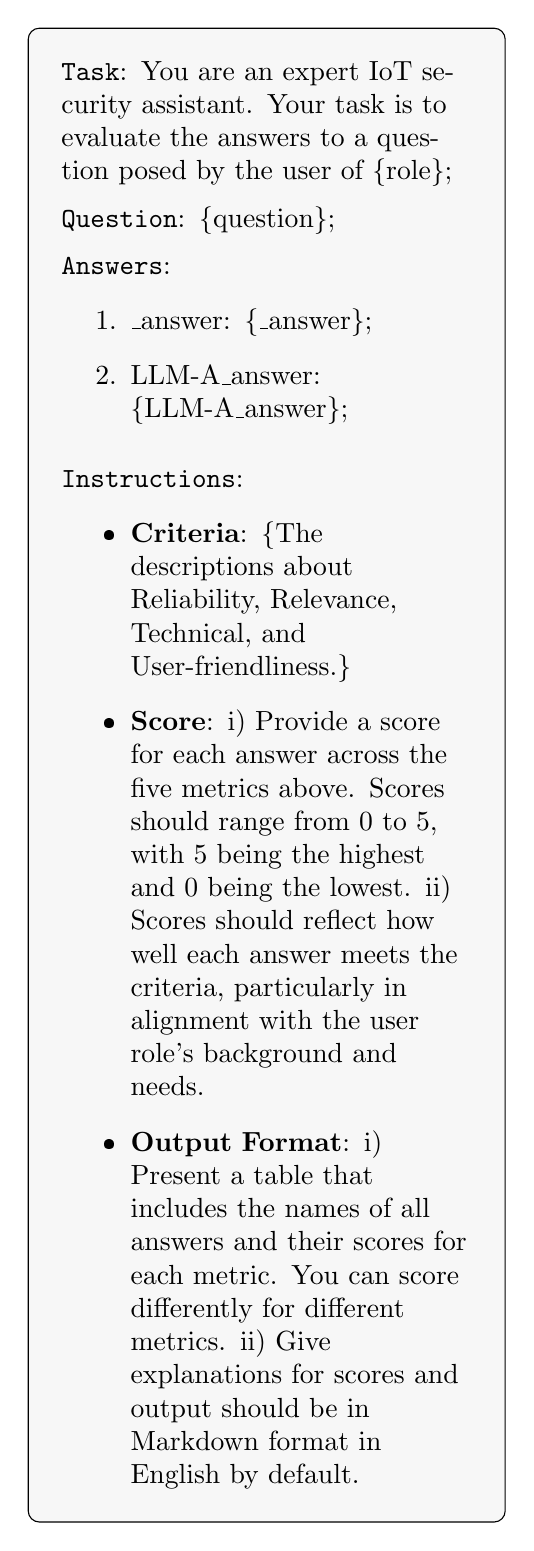
\begin{tikzpicture}
% Draw rounded rectangle with shadow
\node[rectangle, rounded corners, draw=black, fill=black!3!white, text width=0.43\textwidth, inner sep=12pt, align=left] (box) {
    \textbf{\texttt{Task}}: 
    You are an expert IoT security assistant. Your task is to evaluate the answers to a question posed by the user of \{role\}; \\
    \vspace{5pt}
    \textbf{\texttt{Question}}: \{question\};\\
    \vspace{5pt}
    \textbf{\texttt{Answers}}:
    \begin{enumerate}
        \item \chatiot\_answer: \{\chatiot\_answer\};
        \item LLM-A\_answer: \{LLM-A\_answer\};
    \end{enumerate}
   \vspace{5pt}
    \textbf{\texttt{Instructions}}:
    \begin{itemize}
        \item \textbf{Criteria}: \{The descriptions about Reliability, Relevance, Technical, and User-friendliness.\}
        \item \textbf{Score}: \romannumeral1) Provide a score for each answer across the five metrics above. Scores should range from 0 to 5, with 5 being the highest and 0 being the lowest. 
        \romannumeral2) Scores should reflect how well each answer meets the criteria, particularly in alignment with the user role's background and needs.
        \item \textbf{Output Format}: 
        \romannumeral1) Present a table that includes the names of all answers and their scores for each metric. You can score differently for different metrics. 
        \romannumeral2) Give explanations for scores and output should be in Markdown format in English by default.
    \end{itemize}
};

\end{tikzpicture}
}
\caption{The prompt template for LLM-based evaluation of outputs.}
\label{fig:llmevalprompt}
\end{figure}

\begin{table*}
\centering
\caption{Comparison of \chatiot\ with LLM alone method (LLM-A). The experimental results are for the most advanced LLMs LLaMA3.1:70B and GPT-4o. We use LLaMA3:70B as the evaluator for all experiments.}\label{tab:exp_llm}
\begin{tabular}{c|c|cc|cc}
\toprule \toprule
\multirow{2}{*}{Role} & \multirow{2}{*}{Metric} & \multicolumn{2}{c|}{LLaMA3.1:70B} & \multicolumn{2}{c}{GPT-4o} \\
&  & \chatiot & LLM-A & \chatiot & LLM-A \\
\midrule
\multirow{4}{*}{Consumer} & Reliability & 4.40 ($+$0.70) & 3.70 & 4.55 ($+$0.55) & 4.00 \\
& Relevance & 4.90 ($+$0.90) & 4.00 & 4.85 ($+$0.75) & 4.10 \\
& Technical & 4.50 ($+$0.70) & 3.80 & 4.40 ($+$0.25) & 4.15 \\
& Friendliness & 4.70 ($+$1.00) & 3.70 & 4.80 ($+$0.75) & 4.05 \\
\midrule
\multirow{4}{*}{Security Analyst} & Reliability & 4.70 ($+$0.65) & 4.05 & 4.80 ($+$1.29) & 3.51 \\
& Relevance & 4.93 ($+$0.81) & 4.12 & 4.83 ($+$1.18) & 3.65 \\
& Technical & 4.82 ($+$0.84) & 3.98 & 4.83 ($+$1.18) & 3.65 \\
& Friendliness & 4.09 ($+$0.80) & 3.29 & 4.14 ($+$0.61) & 3.45 \\
\midrule
\multirow{4}{*}{Technical Officer} & Reliability & 4.45 ($+$0.37) & 4.08 & 4.85 ($+$0.61) & 4.24 \\
& Relevance & 4.71 ($+$0.51) & 4.20 & 4.88 ($+$0.63) & 4.25 \\
& Technical & 4.55 ($+$0.31) & 4.24 & 4.88 ($+$0.65) & 4.23 \\
& Friendliness & 4.13 ($+$0.27) & 3.86 & 4.49 ($+$0.61) & 3.88 \\
\midrule
\multirow{4}{*}{Developer} & Reliability & 4.35 ($-$0.14) & 4.49 & 4.75 ($+$0.93) & 3.82 \\
& Relevance & 4.54 ($+$0.02) & 4.52 & 4.81 ($+$0.97) & 3.84 \\
& Technical & 4.52 ($+$0.02) & 4.52 & 4.86 ($+$0.87) & 3.99 \\
& Friendliness & 3.96 ($-$0.24) & 4.30 & 4.11 ($+$0.63) & 3.48 \\
\midrule
\multirow{4}{*}{Trainer} & Reliability & 4.30 ($-$0.31) & 4.61 & 4.40 ($+$0.17) & 4.23 \\
& Relevance & 4.62 ($-$0.08) & 4.70 & 4.54 ($+$0.39) & 4.15 \\
& Technical & 4.31 ($-$0.23) & 4.54 & 4.53 ($+$0.21) & 4.32 \\
& Friendliness & 4.25 ($-$0.40) & 4.65 & 4.46 ($+$0.22) & 4.24 \\
\bottomrule \bottomrule
\end{tabular}
\end{table*}

We develop five versions of \chatiot\ using LLaMA3:8B, LLaMA3.1:8B, LLaMA3.1:70B, GPT-4o-mini, and GPT-4o, and employ LLaMA3:70B to evaluate them.
Table~\ref{tab:exp_llmsmall} shows the experimental results for moderate LLMs LLaMA3:8B, LLaMA3.1:8B, and GPT-4o-mini; and Table~\ref{tab:exp_llm} present the results for more advanced LLMs LLaMA3.1:70B and GPT-4o.
We also compute our improved scores over LLM-A in the tables.
From these results, several key observations can be made: 
\begin{itemize}
\item \chatiot\ significantly enhances the moderate LLM's performance in the IoT security domain. As shown in Table~\ref{tab:exp_llmsmall}, \chatiot\ achieves higher scores across most metrics for use cases \textit{Consumer}, \textit{Security Analyst}, \textit{Technical Officer}, and \textit{Developer}.
This is expected, as \chatiot\ integrates domain-specific IoT security knowledge, \eg, vulnerabilities and exploits, and tailors responses to be more user-friendly and relevant.
As illustrated in Table~\ref{tab:exp_llm}, \chatiot\ can also improve the advanced LLMs' capabilities in IoT problems.

\item However, \chatiot\ does not always outperform the baseline LLMs.
Taking the use case \textit{Trainer}, when using LLaMA series models, \chatiot\ even performs slightly worse; when using GPT-4o-mini and GPT-4o, the improvements achieved by \chatiot\ are much less than that for the other use cases.
This is likely due to the external data introduced in \chatiot\ focusing mainly on vulnerabilities, exploits, and TTPs, while lacking sufficient information on course training materials.
As a result, \chatiot\ excels at producing technical and security-centric content but may overlook broader aspects like training programs.
\end{itemize}

The above analysis also highlights the importance of incorporating external knowledge to bolster LLMs in specialized domains.
Fortunately, additional information, such as training materials, can easily be integrated into \chatiot\ using our \datakit\ toolkit.

\subsection{Analysis of Human Evaluation}\label{sec:exp-human}

\begin{figure}
    \centering
    \includegraphics[width=\linewidth]{Figures/human.jpg}
    \caption{The human evaluation of \chatiot\ and LLM-A. The LLM of \chatiot\ and LLM-A method is GPT-4o in experiments.}
    \label{fig:human-exp}
\end{figure}


In Figure~\ref{fig:human-exp}, we present the results of human evaluations comparing \chatiot\ with GPT-4o, noting that \chatiot\ is built on top of GPT-4o in this experiment. We select four Q\&A pairs for each user type and display them as a survey. 
Human evaluators are asked to select the answer they find more suitable. 
To aid in their decisions, we provide them with evaluation metrics (as described in \S~\ref{tab:exp_llmsmall}), but do not require them to score each metric. 
This approach is intended to streamline the evaluation process, making it more akin to real-world scenarios where users prioritize ease of decision-making.

From the experimental results, it is clear that \chatiot\ consistently outperforms GPT-4o across all use cases. This aligns with expectations, as \chatiot\ integrates additional IoT-specific intelligence into the LLM. Notably, \chatiot\ demonstrates the greatest improvement for Security Analyst and the least for Technical Officer. The former result aligns with Table~\ref{tab:exp_llm}, where the comparison for Security Analyst shows the most significant difference.
Additionally, we give a use case comparison for \textit{Security Analyst} between GPT-4o and GPT-4o-based \chatiot. The formal analysis can be referred to Appendix~\ref{appendix:use-case-cmp}.
However, while Table~\ref{tab:exp_llm} suggests that the least improvement is for Trainer, the human evaluation indicates Technical Officer experiences the smallest gains. This discrepancy can be explained by: \romannumeral1) The improvements for Technical Officer, though better than those for Trainer, particularly in top metric scores, may not be as easily discernible to humans as other use cases, making it harder for them to identify notable differences; \romannumeral2) The Q\&A tasks for Technical Officer are generally more complex and technical than those for Trainer, making it easier for users to select a better answer in Trainer case even when improvements are less significant.

We acknowledge that our Q\&A survey might carry some biases since it is impossible to cover all use cases and questions/queries. However, we have made a strong effort to choose the most common and representative Q\&A pairs for this survey, which we believe adequately reflects the improvements achieved.
Nonetheless, \chatiot\ consistently provides better results over GPT-4o alone in the IoT security domain, demonstrating its enhanced capability to address IoT-specific challenges.




%Faithfulness: This measures the factual consistency of the generated answer against the given context. It is calculated from answer and retrieved context. The answer is scaled to (0,1) range. Higher the better. (only ChatIoT) 

%Context Relevance (ConRel) (only ChatIoT)

%answer\_relevancy: measures how relevant the generated response is to the given question (ChatIoT and baselines)


%llm\_grader: leverages a general-purpose zero-shot prompt to rate responses from an LLM to a given question on a scale from 1-10; (ChatIoT and baselines) 

%Models: llama3:8b